% !TeX root = RJwrapper.tex
\title{Rain in Australia. Classification Prediction Model}
\author{by Sumaira Afzal, Viraja Ketkar, Murlidhar Loka, Vadim Spirkov}

\maketitle

\abstract{%
Many native cultures comprise an institution of ``rainmakers'' -- people
who would not as much invoke the rains, but anticipate them based on
ethno-meteorology. The forecasting was based on skillful art of
observing the natural environment as expressed in the timing or
flowering of plants, hatching of insects, arrival of migratory birds,
etc., which enables farmers to make adjustments in farming calendar and
crop selection types in any given season. This indigenous knowledge was
often passed down from one generation to the other. We are going to
employ CRISP-DM framework (Ref: \cite{mining}) along with the latest
scientific methods and prediction algorithms to achieve the same very
goal without thorough knowledge of forces of nature, hopefully with the
same accuracy as the aboriginal people.
}

% Any extra LaTeX you need in the preamble

\hypertarget{background}{%
\subsection{Background}\label{background}}

Weather forecasting is a complex and often challenging skill that
involves observing and processing vast amounts of data. Weather systems
can range from small, short lived thunderstorms only a few kilometers in
diameter that last a couple hours to large scale rain and snow storms up
to a thousand kilometers in diameter and lasting for days.

A very important component of modern weather forecasting is the use of
numerical weather prediction (NWP) models. In the last years, the
forecast quality of those models constantly improved, mostly due to
major improvements in high performance computing. NWP focuses on taking
current observations of weather and processing these data with computer
models to forecast the future state of weather. Knowing the current
state of the weather is just as important as the numerical computer
models processing the data. Current weather observations serve as input
to the numerical computer models through a process known as data
assimilation to produce outputs of temperature, precipitation, and
hundreds of other meteorological elements from the oceans to the top of
the atmosphere. \cite{ams}

\hypertarget{objective}{%
\subsection{Objective}\label{objective}}

The objective of this research is to find a supervised, binary
classification model that would provide accurate forecast of the rain in
Australia next day, having today's weather observations and historical
data. In addition to being accurate the model should be easily
interpretable and flexible enough to accept limited number of input
features without diminishing its prediction power.

\hypertarget{data-analysis}{%
\section{Data Analysis}\label{data-analysis}}

The data set we are going to use for our research contains daily weather
observations from numerous Australian weather stations collected from
2007 till 2017. There are over 142000 records. It has been sourced from
\href{https://www.kaggle.com/jsphyg/weather-dataset-rattle-package}{Kaggle}

\hypertarget{data-dictionary}{%
\subsection{Data Dictionary}\label{data-dictionary}}

We exclude the variable \emph{Risk-MM} when training your binary
classification model. If we don't exclude it, you will leak the answers
to our model and reduce its predictability

\begin{longtable}[]{@{}ll@{}}
\toprule
\begin{minipage}[b]{0.52\columnwidth}\raggedright
Column Name\strut
\end{minipage} & \begin{minipage}[b]{0.43\columnwidth}\raggedright
Column Description\strut
\end{minipage}\tabularnewline
\midrule
\endhead
\begin{minipage}[t]{0.52\columnwidth}\raggedright
Date\strut
\end{minipage} & \begin{minipage}[t]{0.43\columnwidth}\raggedright
Date of observation\strut
\end{minipage}\tabularnewline
\begin{minipage}[t]{0.52\columnwidth}\raggedright
Location\strut
\end{minipage} & \begin{minipage}[t]{0.43\columnwidth}\raggedright
Common name of the location of the weather station\strut
\end{minipage}\tabularnewline
\begin{minipage}[t]{0.52\columnwidth}\raggedright
MinTemp\strut
\end{minipage} & \begin{minipage}[t]{0.43\columnwidth}\raggedright
Minimum temperature in degrees Celsius\strut
\end{minipage}\tabularnewline
\begin{minipage}[t]{0.52\columnwidth}\raggedright
MaxTemp\strut
\end{minipage} & \begin{minipage}[t]{0.43\columnwidth}\raggedright
Maximum temperature in degrees Celsius\strut
\end{minipage}\tabularnewline
\begin{minipage}[t]{0.52\columnwidth}\raggedright
Rainfall\strut
\end{minipage} & \begin{minipage}[t]{0.43\columnwidth}\raggedright
Amount of rainfall recorded for the day in mm\strut
\end{minipage}\tabularnewline
\begin{minipage}[t]{0.52\columnwidth}\raggedright
Evaporation\strut
\end{minipage} & \begin{minipage}[t]{0.43\columnwidth}\raggedright
So-called Class A pan evaporation (mm) in the 24 hours to 9am\strut
\end{minipage}\tabularnewline
\begin{minipage}[t]{0.52\columnwidth}\raggedright
Sunshine\strut
\end{minipage} & \begin{minipage}[t]{0.43\columnwidth}\raggedright
Number of hours of bright sunshine in the day\strut
\end{minipage}\tabularnewline
\begin{minipage}[t]{0.52\columnwidth}\raggedright
WindGustDir\strut
\end{minipage} & \begin{minipage}[t]{0.43\columnwidth}\raggedright
Direction of the strongest wind gust in the 24 hours to midnight\strut
\end{minipage}\tabularnewline
\begin{minipage}[t]{0.52\columnwidth}\raggedright
WindGustSpeed\strut
\end{minipage} & \begin{minipage}[t]{0.43\columnwidth}\raggedright
Speed (km/h) of the strongest wind gust in the 24 hours to
midnight\strut
\end{minipage}\tabularnewline
\begin{minipage}[t]{0.52\columnwidth}\raggedright
WindDir9amDirection\strut
\end{minipage} & \begin{minipage}[t]{0.43\columnwidth}\raggedright
Of the wind at 9am\strut
\end{minipage}\tabularnewline
\begin{minipage}[t]{0.52\columnwidth}\raggedright
WindDir3pmDirection\strut
\end{minipage} & \begin{minipage}[t]{0.43\columnwidth}\raggedright
Of the wind at 3pm\strut
\end{minipage}\tabularnewline
\begin{minipage}[t]{0.52\columnwidth}\raggedright
WindSpeed9amWind\strut
\end{minipage} & \begin{minipage}[t]{0.43\columnwidth}\raggedright
Wind speed (km/hr) averaged over 10 minutes prior to 9am\strut
\end{minipage}\tabularnewline
\begin{minipage}[t]{0.52\columnwidth}\raggedright
WindSpeed3pmWind\strut
\end{minipage} & \begin{minipage}[t]{0.43\columnwidth}\raggedright
Wind Speed (km/hr) averaged over 10 minutes prior to 3pm\strut
\end{minipage}\tabularnewline
\begin{minipage}[t]{0.52\columnwidth}\raggedright
Humidity9amHumidity\strut
\end{minipage} & \begin{minipage}[t]{0.43\columnwidth}\raggedright
Humidity (percent) at 9am\strut
\end{minipage}\tabularnewline
\begin{minipage}[t]{0.52\columnwidth}\raggedright
Humidity3pmHumidity\strut
\end{minipage} & \begin{minipage}[t]{0.43\columnwidth}\raggedright
Humidity (percent) at 3pm\strut
\end{minipage}\tabularnewline
\begin{minipage}[t]{0.52\columnwidth}\raggedright
Pressure9amAtmospheric\strut
\end{minipage} & \begin{minipage}[t]{0.43\columnwidth}\raggedright
Pressure (hpa) reduced to mean sea level at 9am\strut
\end{minipage}\tabularnewline
\begin{minipage}[t]{0.52\columnwidth}\raggedright
Pressure3pmAtmospheric\strut
\end{minipage} & \begin{minipage}[t]{0.43\columnwidth}\raggedright
Pressure (hpa) reduced to mean sea level at 3pm\strut
\end{minipage}\tabularnewline
\begin{minipage}[t]{0.52\columnwidth}\raggedright
Cloud9amFraction\strut
\end{minipage} & \begin{minipage}[t]{0.43\columnwidth}\raggedright
Area of sky obscured by cloud at 9am. This is measured in ``oktas'',
which are a unit of eights. It records how many eights of the sky are
obscured by cloud. A 0 measure indicates completely clear sky whilst an
8 indicates that it is completely overcast\strut
\end{minipage}\tabularnewline
\begin{minipage}[t]{0.52\columnwidth}\raggedright
Cloud3pmFraction\strut
\end{minipage} & \begin{minipage}[t]{0.43\columnwidth}\raggedright
Area of sky obscured by cloud (in ``oktas'': eighths) at 3pm. See
Cloud9am for a description of the values\strut
\end{minipage}\tabularnewline
\begin{minipage}[t]{0.52\columnwidth}\raggedright
Temp9amTemperature\strut
\end{minipage} & \begin{minipage}[t]{0.43\columnwidth}\raggedright
Temperature (degrees C) at 9am\strut
\end{minipage}\tabularnewline
\begin{minipage}[t]{0.52\columnwidth}\raggedright
Temp3pmTemperature\strut
\end{minipage} & \begin{minipage}[t]{0.43\columnwidth}\raggedright
Temperature (degrees C) at 3pm\strut
\end{minipage}\tabularnewline
\begin{minipage}[t]{0.52\columnwidth}\raggedright
RainTodayBoolean\strut
\end{minipage} & \begin{minipage}[t]{0.43\columnwidth}\raggedright
Rainy today. 1 if precipitation (mm) in the 24 hours to 9am exceeds 1mm,
otherwise 0\strut
\end{minipage}\tabularnewline
\begin{minipage}[t]{0.52\columnwidth}\raggedright
RISK\_MM\strut
\end{minipage} & \begin{minipage}[t]{0.43\columnwidth}\raggedright
Amount of rain. A kind of measure of the ``risk''. This column is
redundant and will be dropped\strut
\end{minipage}\tabularnewline
\begin{minipage}[t]{0.52\columnwidth}\raggedright
\textbf{RainTomorrow}\strut
\end{minipage} & \begin{minipage}[t]{0.43\columnwidth}\raggedright
\textbf{Class label. Will it rain tomorrow?}\strut
\end{minipage}\tabularnewline
\bottomrule
\end{longtable}

\hypertarget{data-exploration}{%
\subsection{Data Exploration}\label{data-exploration}}

Let's take a close look at the data set. We start with loading weather
observations from the file into a data frame. We remove \emph{RISK\_MM}
as explained and convert \emph{Date} column to ``date''" data type.

\begin{Schunk}
\begin{Sinput}
weatherData = read.csv("../data/weatherAUS.csv", header = TRUE, na.strings = c("NA","","#NA"),sep=",")
weatherData = subset(weatherData, select = -RISK_MM)
weatherData$Date = as.Date(as.character(weatherData$Date),"%Y-%m-%d")
\end{Sinput}
\end{Schunk}

Now we are going to load coordinates of the weather stations and have a
bird-eye view of the weather station locations.

\begin{Schunk}
\begin{figure}[H]

{\centering 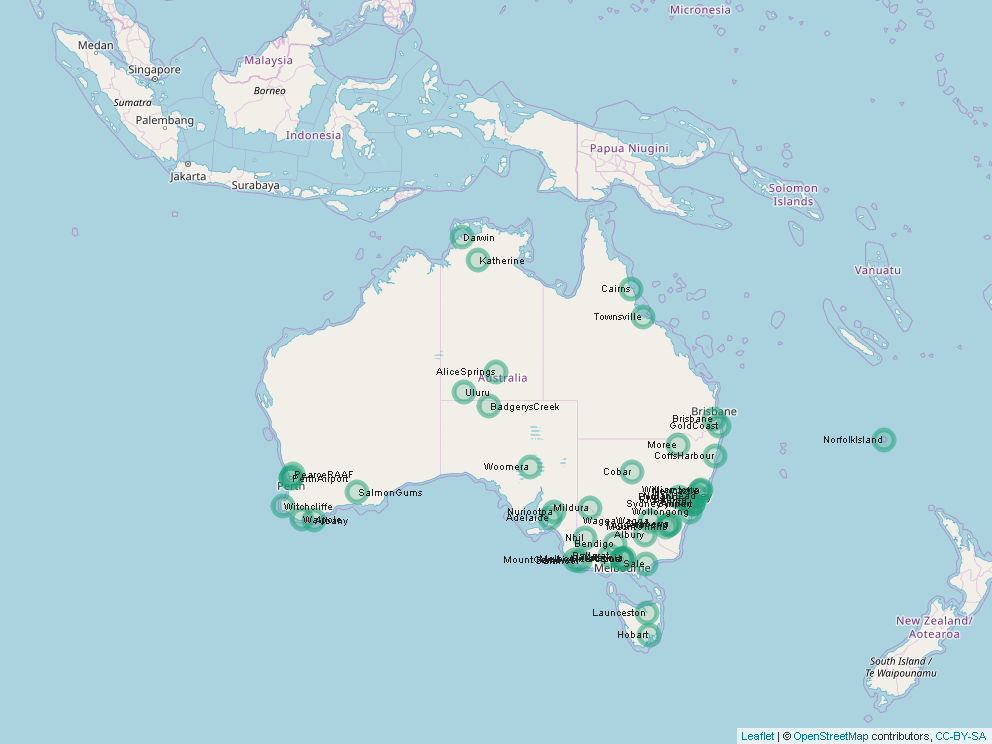
\includegraphics[width=1.1\linewidth]{images/weatherStations} 

}

\caption[Australian Weather Stations]{Australian Weather Stations}\label{fig:map}
\end{figure}
\end{Schunk}

To have the full picture of the data let's print the data summary and
sample.

\begin{table}[ht]
\centering
\scalebox{0.7}{
\begin{tabular}{llllllll}
  \hline
     Date &     Location &    MinTemp &    MaxTemp &    Rainfall &  Evaporation &    Sunshine &  WindGustDir \\ 
  \hline
Min.   :2007-11-01   & Canberra:  3418   & Min.   :-8.50   & Min.   :-4.80   & Min.   :  0.00   & Min.   :  0.00   & Min.   : 0.00   & W      : 9780   \\ 
  1st Qu.:2011-01-06   & Sydney  :  3337   & 1st Qu.: 7.60   & 1st Qu.:17.90   & 1st Qu.:  0.00   & 1st Qu.:  2.60   & 1st Qu.: 4.90   & SE     : 9309   \\ 
  Median :2013-05-27   & Perth   :  3193   & Median :12.00   & Median :22.60   & Median :  0.00   & Median :  4.80   & Median : 8.50   & E      : 9071   \\ 
  Mean   :2013-04-01   & Darwin  :  3192   & Mean   :12.19   & Mean   :23.23   & Mean   :  2.35   & Mean   :  5.47   & Mean   : 7.62   & N      : 9033   \\ 
  3rd Qu.:2015-06-12   & Hobart  :  3188   & 3rd Qu.:16.80   & 3rd Qu.:28.20   & 3rd Qu.:  0.80   & 3rd Qu.:  7.40   & 3rd Qu.:10.60   & SSE    : 8993   \\ 
  Max.   :2017-06-25   & Brisbane:  3161   & Max.   :33.90   & Max.   :48.10   & Max.   :371.00   & Max.   :145.00   & Max.   :14.50   & (Other):86677   \\ 
   & (Other) :122704   & NA's   :637   & NA's   :322   & NA's   :1406   & NA's   :60843   & NA's   :67816   & NA's   : 9330   \\ 
   \hline
\end{tabular}
}
\end{table}
\begin{table}[ht]
\centering
\scalebox{0.7}{
\begin{tabular}{llllllll}
  \hline
WindGustSpeed &   WindDir9am &   WindDir3pm &  WindSpeed9am &  WindSpeed3pm &  Humidity9am &  Humidity3pm &  Pressure9am \\ 
  \hline
Min.   :  6.00   & N      :11393   & SE     :10663   & Min.   :  0   & Min.   : 0.00   & Min.   :  0.00   & Min.   :  0.00   & Min.   : 980.5   \\ 
  1st Qu.: 31.00   & SE     : 9162   & W      : 9911   & 1st Qu.:  7   & 1st Qu.:13.00   & 1st Qu.: 57.00   & 1st Qu.: 37.00   & 1st Qu.:1012.9   \\ 
  Median : 39.00   & E      : 9024   & S      : 9598   & Median : 13   & Median :19.00   & Median : 70.00   & Median : 52.00   & Median :1017.6   \\ 
  Mean   : 39.98   & SSE    : 8966   & WSW    : 9329   & Mean   : 14   & Mean   :18.64   & Mean   : 68.84   & Mean   : 51.48   & Mean   :1017.7   \\ 
  3rd Qu.: 48.00   & NW     : 8552   & SW     : 9182   & 3rd Qu.: 19   & 3rd Qu.:24.00   & 3rd Qu.: 83.00   & 3rd Qu.: 66.00   & 3rd Qu.:1022.4   \\ 
  Max.   :135.00   & (Other):85083   & (Other):89732   & Max.   :130   & Max.   :87.00   & Max.   :100.00   & Max.   :100.00   & Max.   :1041.0   \\ 
  NA's   :9270   & NA's   :10013   & NA's   : 3778   & NA's   :1348   & NA's   :2630   & NA's   :1774   & NA's   :3610   & NA's   :14014   \\ 
   \hline
\end{tabular}
}
\end{table}
\begin{table}[ht]
\centering
\scalebox{0.7}{
\begin{tabular}{lllllll}
  \hline
 Pressure3pm &    Cloud9am &    Cloud3pm &    Temp9am &    Temp3pm & RainToday & RainTomorrow \\ 
  \hline
Min.   : 977.1   & Min.   :0.00   & Min.   :0.0   & Min.   :-7.20   & Min.   :-5.40   & No  :109332   & No :110316   \\ 
  1st Qu.:1010.4   & 1st Qu.:1.00   & 1st Qu.:2.0   & 1st Qu.:12.30   & 1st Qu.:16.60   & Yes : 31455   & Yes: 31877   \\ 
  Median :1015.2   & Median :5.00   & Median :5.0   & Median :16.70   & Median :21.10   & NA's:  1406   &  \\ 
  Mean   :1015.3   & Mean   :4.44   & Mean   :4.5   & Mean   :16.99   & Mean   :21.69   &  &  \\ 
  3rd Qu.:1020.0   & 3rd Qu.:7.00   & 3rd Qu.:7.0   & 3rd Qu.:21.60   & 3rd Qu.:26.40   &  &  \\ 
  Max.   :1039.6   & Max.   :9.00   & Max.   :9.0   & Max.   :40.20   & Max.   :46.70   &  &  \\ 
  NA's   :13981   & NA's   :53657   & NA's   :57094   & NA's   :904   & NA's   :2726   &  &  \\ 
   \hline
\end{tabular}
}
\caption{\tt Weather Obesrvations Data Summary} 
\label{data_head}
\end{table}

\newpage
\begin{table}[ht]
\centering
\scalebox{0.6}{
\begin{tabular}{rrlrrrrrlrllr}
  \hline
 & Date & Location & MinTemp & MaxTemp & Rainfall & Evaporation & Sunshine & WindGustDir & WindGustSpeed & WindDir9am & WindDir3pm & WindSpeed9am \\ 
  \hline
1 & 14214.00 & Albury & 13.40 & 22.90 & 0.60 &  &  & W &  44 & W & WNW &  20 \\ 
  2 & 14215.00 & Albury & 7.40 & 25.10 & 0.00 &  &  & WNW &  44 & NNW & WSW &   4 \\ 
  3 & 14216.00 & Albury & 12.90 & 25.70 & 0.00 &  &  & WSW &  46 & W & WSW &  19 \\ 
  4 & 14217.00 & Albury & 9.20 & 28.00 & 0.00 &  &  & NE &  24 & SE & E &  11 \\ 
  5 & 14218.00 & Albury & 17.50 & 32.30 & 1.00 &  &  & W &  41 & ENE & NW &   7 \\ 
  6 & 14219.00 & Albury & 14.60 & 29.70 & 0.20 &  &  & WNW &  56 & W & W &  19 \\ 
  7 & 14220.00 & Albury & 14.30 & 25.00 & 0.00 &  &  & W &  50 & SW & W &  20 \\ 
  8 & 14221.00 & Albury & 7.70 & 26.70 & 0.00 &  &  & W &  35 & SSE & W &   6 \\ 
  9 & 14222.00 & Albury & 9.70 & 31.90 & 0.00 &  &  & NNW &  80 & SE & NW &   7 \\ 
  10 & 14223.00 & Albury & 13.10 & 30.10 & 1.40 &  &  & W &  28 & S & SSE &  15 \\ 
   \hline
\end{tabular}
}
\end{table}
\begin{table}[ht]
\centering
\scalebox{0.6}{
\begin{tabular}{rrrrrrrrrll}
  \hline
WindSpeed3pm & Humidity9am & Humidity3pm & Pressure9am & Pressure3pm & Cloud9am & Cloud3pm & Temp9am & Temp3pm & RainToday & RainTomorrow \\ 
  \hline
 24 &  71 &  22 & 1007.70 & 1007.10 &   8 &  & 16.90 & 21.80 & No & No \\ 
   22 &  44 &  25 & 1010.60 & 1007.80 &  &  & 17.20 & 24.30 & No & No \\ 
   26 &  38 &  30 & 1007.60 & 1008.70 &  &   2 & 21.00 & 23.20 & No & No \\ 
    9 &  45 &  16 & 1017.60 & 1012.80 &  &  & 18.10 & 26.50 & No & No \\ 
   20 &  82 &  33 & 1010.80 & 1006.00 &   7 &   8 & 17.80 & 29.70 & No & No \\ 
   24 &  55 &  23 & 1009.20 & 1005.40 &  &  & 20.60 & 28.90 & No & No \\ 
   24 &  49 &  19 & 1009.60 & 1008.20 &   1 &  & 18.10 & 24.60 & No & No \\ 
   17 &  48 &  19 & 1013.40 & 1010.10 &  &  & 16.30 & 25.50 & No & No \\ 
   28 &  42 &   9 & 1008.90 & 1003.60 &  &  & 18.30 & 30.20 & No & Yes \\ 
   11 &  58 &  27 & 1007.00 & 1005.70 &  &  & 20.10 & 28.20 & Yes & No \\ 
   \hline
\end{tabular}
}
\caption{\tt Weather Obesrvations Data Sample} 
\label{data_head}
\end{table}

Next set of plots renders distribution of a few important features.
Overall all the features of the data set could be split into a few
groups: temperature observations, humidity, wind speed, wind direction,
cloud coverage, pressure, evaporation and sunshine. We picked one
parameter from each group assuming that they represent well the
remaining group attributes.

\begin{Schunk}
\begin{figure}[H]

{\centering \includegraphics{main_files/figure-latex/feature_distribution-1} 

}

\caption[ Distribution of Important Features]{ Distribution of Important Features}\label{fig:feature_distribution}
\end{figure}
\end{Schunk}

\hypertarget{missing-data}{%
\subsubsection{Missing Data}\label{missing-data}}

Data summary shows that some features miss data. Some data losses are
very significant. We are going to identify what data is missing and if
it is feasible to recover the missing data.

\begin{Schunk}
\begin{Sinput}
sort(colSums(is.na(weatherData)), decreasing = T)
\end{Sinput}
\begin{Soutput}
#>      Sunshine   Evaporation      Cloud3pm      Cloud9am   Pressure9am 
#>         67816         60843         57094         53657         14014 
#>   Pressure3pm    WindDir9am   WindGustDir WindGustSpeed    WindDir3pm 
#>         13981         10013          9330          9270          3778 
#>   Humidity3pm       Temp3pm  WindSpeed3pm   Humidity9am      Rainfall 
#>          3610          2726          2630          1774          1406 
#>     RainToday  WindSpeed9am       Temp9am       MinTemp       MaxTemp 
#>          1406          1348           904           637           322 
#>          Date      Location  RainTomorrow 
#>             0             0             0
\end{Soutput}
\end{Schunk}

To speed up data processing and plot rendering we are going to use a
data sample. For population of 142K observations, 30K sample size would
be sufficient for 99\% confidence level with the confidence interval 1.

\begin{Schunk}
\begin{Sinput}
weatherSample = sample_n(weatherData, SampleSize)
aggr(weatherSample, numbers = F, prop = T, col = mainPalette, sortVars = T, bars = F, varheight = T)
\end{Sinput}
\begin{figure}[H]

{\centering \includegraphics{main_files/figure-latex/plot_aggr_missing-1} 

}

\caption[Missing Data Summary]{Missing Data Summary}\label{fig:plot_aggr_missing}
\end{figure}
\begin{Soutput}
#> 
#>  Variables sorted by number of missings: 
#>       Variable       Count
#>       Sunshine 0.477500000
#>    Evaporation 0.429600000
#>       Cloud3pm 0.401966667
#>       Cloud9am 0.379733333
#>    Pressure9am 0.100133333
#>    Pressure3pm 0.099833333
#>     WindDir9am 0.071866667
#>    WindGustDir 0.065633333
#>  WindGustSpeed 0.065033333
#>     WindDir3pm 0.027733333
#>    Humidity3pm 0.025900000
#>        Temp3pm 0.019400000
#>   WindSpeed3pm 0.019100000
#>    Humidity9am 0.013400000
#>       Rainfall 0.010633333
#>   WindSpeed9am 0.010633333
#>      RainToday 0.010633333
#>        Temp9am 0.006966667
#>        MinTemp 0.004566667
#>        MaxTemp 0.002600000
#>           Date 0.000000000
#>       Location 0.000000000
#>   RainTomorrow 0.000000000
\end{Soutput}
\end{Schunk}

As demonstrated in Figure \ref{fig:plot_aggr_missing} \emph{Sunshine},
\emph{Evaporation} and \emph{Clouds} attributes suffer the loss of data
between \textbf{48\%} and \textbf{38\%}. This is significant! Since we
are dealing with the weather we should be observing cyclical patterns.
The next group of plots illustrate missing data distribution for the
most damaged features. We employ VIM (Ref: \cite{vim}) package to plot
the missing data.

\begin{Schunk}
\begin{figure}[H]

{\centering \includegraphics{main_files/figure-latex/plot_margin1-1} 

}

\caption[Date/Evaporation Margin Plot]{Date/Evaporation Margin Plot}\label{fig:plot_margin1}
\end{figure}
\end{Schunk}

\begin{Schunk}
\begin{figure}[H]

{\centering \includegraphics{main_files/figure-latex/plot_margin2-1} 

}

\caption[Date/ Sunshine Margin Plot]{Date/ Sunshine Margin Plot}\label{fig:plot_margin2}
\end{figure}
\end{Schunk}

\begin{Schunk}
\begin{figure}[H]

{\centering \includegraphics{main_files/figure-latex/plot_margin3-1} 

}

\caption[Date/ Pressure3pm Margin Plot]{Date/ Pressure3pm Margin Plot}\label{fig:plot_margin3}
\end{figure}
\end{Schunk}

So what do the margin plots tell us? First of all let's take a look at
\emph{Date} axis. The \emph{Date} has been converted to number to ensure
continuous flow of the data. All features we picked exhibit cyclical
pattern as expected. Along the vertical axis we observe the box plot of
the respective feature. \emph{Evaporaton} data is quite remarkable
(Figure \ref{fig:plot_margin1}); it has very narrow distribution and a
lot of so-called outliers. Though the forces of nature follow seasonal
patters they often exhibit wide range of seasonal anomalies, which the
plots highlight. Thus we opt to keep the data as is. The distribution of
the missing data of a given feature is depicted along the horizontal
axis. In all three cases the missing data is randomly distributed over
the observed date range. Along the horizontal axis we may see the box
plots of the date and a given feature. Pressure readings at 9 AM
\emph{Presure9am} (Figure \ref{fig:plot_margin3}) distributed evenly
across the observed date range. \emph{Evaporation} and \emph{Sunshine}
exhibit more data losses towards the end of the observed period.

The next plot examines another dimension of the missing data, namely
missing date grouped by location.

\begin{Schunk}
\begin{figure}[H]

{\centering \includegraphics{main_files/figure-latex/plot_missLocation-1} 

}

\caption[Missing Data By Location]{Missing Data By Location}\label{fig:plot_missLocation}
\end{figure}
\end{Schunk}

Figure \ref{fig:plot_missLocation} shows that on average a location
misses \textbf{6460} observations. This is significant! Though if we
take a second look at the weather station map \ref{fig:map} we would see
that Mount Gini (the station that misses the most data), Bendigo and
Ballarat are close to Melbrun, where the staff kept observing data on
regular basis. Newcastle to Sydney and so on\ldots{} Thus knowing that
the stations are relatively close geographically we could potentially
employ the weather reading collected by one station to approximate the
missing data of the other station, provided they are located nearby.

\hypertarget{data-correlation-and-other-observations}{%
\subsubsection{Data correlation and other
observations}\label{data-correlation-and-other-observations}}

Let's examine how the features are correlated to each other. Knowing
weather we can make an assumption that the temperature features should
be highly correlated, as well as pressure, wind speed, clouds and
humidity groups.

\begin{Schunk}
\begin{figure}[H]

{\centering \includegraphics[width=1.1\linewidth]{main_files/figure-latex/plot_corr-1} 

}

\caption[Data Correlation]{Data Correlation}\label{fig:plot_corr}
\end{figure}
\end{Schunk}

Figure \ref{fig:plot_corr} confirms our initial guess. This observation
will help us to eliminate redundant features later when we get to the
point of selecting useful predictors for our model.

\hypertarget{takeaways-from-data-exploration-excersize}.
  \item
    \emph{Evaporation} \textbf{43\%}.
  \item
    \emph{Cloud} group (\textbf{40\%} and \textbf{38\%} respectively).
  \end{itemize}
\item
  The rest of the features exhibit medium to minor data losses, where
  \emph{Pressure} group leads the way with 10\%
\item
  The missing data is distributed randomly over the observed time frame
  (Figures \ref{fig:plot_margin1}, \ref{fig:plot_margin2},
  \ref{fig:plot_margin3}).
\item
  We also witnessed that some weather stations recorded less data and
  some were almost prefect at record keeping (Figure
  \ref{fig:plot_missLocation}). Luckily majority of the weather stations
  situate relatively close to each other (see figure \ref{fig:map}).
  Thus if a station has data gaps the neighboring station data could be
  used to approximate the missing data with plausible accuracy.
\item
  We have also noticed that many features are either positively or
  negatively correlated (Figure \ref{fig:plot_corr}), where

  \begin{itemize}
  \tightlist
  \item
    \emph{MaxTemp}, \emph{Temp3pm} and \emph{Temp9am} exhibit
    correlation of \textbf{0.86} to \textbf{0.98}.
  \item
    \emph{Pressure9am} and \emph{Pressure3pm} have correlation
    coefficient of \textbf{0.96}.
  \item
    \emph{Sunshine} and \emph{Cloud} group correlated negatively with
    coefficient of \textbf{-0.7}.
  \item
    \emph{Rainfall} feature is of particular interest since this is what
    we are trying to predict. Unfortunately it does not demonstrate any
    strong correlations with any other features.
  \end{itemize}
\item
  Examining the data we have also seen seasonal patterns and the data
  that fall outside of the normal distribution range by far (outliers).
  Those are anomalies of nature which we opt to keep.
\item
  The last but not least the target feature \emph{RainTomorrow} (the
  value we are trying to predict) is unbalanced. So we are dealing with
  unbalanced data set. See Figure \ref{fig:feature_distribution}.
\end{itemize}

\hypertarget{data-preparation}{%
\subsection{Data Preparation}\label{data-preparation}}

Data exploration confirmed that despite significant data loss we should
be able to impute missing data with high degree of accuracy.

\hypertarget{data-imputing}{%
\subsubsection{Data Imputing}\label{data-imputing}}

To impute the missing data we employ \textbf{MICE} package (Ref:
\cite{mice}). Our imputation strategy is to employ \textbf{Predictive
mean matching} model. It is a robust, fast imputation algorithm that
works with numeric values. Prior to applying the algorithm we have to do
some data transformations, which will

\begin{itemize}
\tightlist
\item
  Increase imputation processing speed.
\item
  Improve model training performance and hopefully accuracy.
\end{itemize}

First of all let's get rid of \emph{Date} column. Outside of the
presentation it does not carry too mach information. What would be
useful indeed is a feature that captures seasonal fluctuations. That
would bee \emph{month} and \emph{day} combined, giving us year-round
(365) days of observations.

Secondly we convert \emph{Location} categorical feature (Factor) to
plain numeric column. Indeed there are 49 locations. If we dummy-encode
locations how much would it improve the performance of the imputation
algorithm and the processing speed (we are talking about 49 new
columns\ldots{})? We believe it is more harmful than helpful. Thus we go
for numeric presentation. Another topic for pondering is whether we
shall employ weather station coordinates\ldots{} After some deliberation
we can conclude that the coordinates will not add much knowledge in the
context of the model training. But they will certainly break the
categorical nature of the locations. Each coordinates have 4 - 6 decimal
places, which effectively makes them continuous. So we stick with
numeric presentation of the locations.

We also convert other factor data types to numbers in order to make
\emph{MICE} pick \textbf{Predictive mean matching} model (vs
\emph{Multinomial logit} model, that exhibits poor speed and low
performance dealing with the categorical features of 20 levels or more).

This is our original set.

\begin{Schunk}
\begin{Soutput}
#> 'data.frame':    142193 obs. of  23 variables:
#>  $ Date         : Date, format: "2008-12-01" "2008-12-02" ...
#>  $ Location     : Factor w/ 49 levels "Adelaide","Albany",..: 3 3 3 3 3 3 3 3 3 3 ...
#>  $ MinTemp      : num  13.4 7.4 12.9 9.2 17.5 14.6 14.3 7.7 9.7 13.1 ...
#>  $ MaxTemp      : num  22.9 25.1 25.7 28 32.3 29.7 25 26.7 31.9 30.1 ...
#>  $ Rainfall     : num  0.6 0 0 0 1 0.2 0 0 0 1.4 ...
#>  $ Evaporation  : num  NA NA NA NA NA NA NA NA NA NA ...
#>  $ Sunshine     : num  NA NA NA NA NA NA NA NA NA NA ...
#>  $ WindGustDir  : Factor w/ 16 levels "E","ENE","ESE",..: 14 15 16 5 14 15 14 14 7 14 ...
#>  $ WindGustSpeed: int  44 44 46 24 41 56 50 35 80 28 ...
#>  $ WindDir9am   : Factor w/ 16 levels "E","ENE","ESE",..: 14 7 14 10 2 14 13 11 10 9 ...
#>  $ WindDir3pm   : Factor w/ 16 levels "E","ENE","ESE",..: 15 16 16 1 8 14 14 14 8 11 ...
#>  $ WindSpeed9am : int  20 4 19 11 7 19 20 6 7 15 ...
#>  $ WindSpeed3pm : int  24 22 26 9 20 24 24 17 28 11 ...
#>  $ Humidity9am  : int  71 44 38 45 82 55 49 48 42 58 ...
#>  $ Humidity3pm  : int  22 25 30 16 33 23 19 19 9 27 ...
#>  $ Pressure9am  : num  1008 1011 1008 1018 1011 ...
#>  $ Pressure3pm  : num  1007 1008 1009 1013 1006 ...
#>  $ Cloud9am     : int  8 NA NA NA 7 NA 1 NA NA NA ...
#>  $ Cloud3pm     : int  NA NA 2 NA 8 NA NA NA NA NA ...
#>  $ Temp9am      : num  16.9 17.2 21 18.1 17.8 20.6 18.1 16.3 18.3 20.1 ...
#>  $ Temp3pm      : num  21.8 24.3 23.2 26.5 29.7 28.9 24.6 25.5 30.2 28.2 ...
#>  $ RainToday    : Factor w/ 2 levels "No","Yes": 1 1 1 1 1 1 1 1 1 2 ...
#>  $ RainTomorrow : Factor w/ 2 levels "No","Yes": 1 1 1 1 1 1 1 1 2 1 ...
\end{Soutput}
\end{Schunk}

Transformation.

\begin{Schunk}
\begin{Sinput}
data = mutate(weatherData,MMDD = as.numeric( format(Date, "%m%d")),Location = unclass(Location),   
              WindGustDir = unclass(WindGustDir), 
              WindDir9am = unclass(WindDir9am), WindDir3pm = unclass(WindDir3pm),
              RainToday = unclass(RainToday)-1, RainTomorrow = unclass(RainTomorrow)-1)
data =  subset(data, select = -Date)
\end{Sinput}
\end{Schunk}

Resulting data frame structure.

\begin{Schunk}
\begin{Soutput}
#> 'data.frame':    142193 obs. of  23 variables:
#>  $ Location     : int  3 3 3 3 3 3 3 3 3 3 ...
#>  $ MinTemp      : num  13.4 7.4 12.9 9.2 17.5 14.6 14.3 7.7 9.7 13.1 ...
#>  $ MaxTemp      : num  22.9 25.1 25.7 28 32.3 29.7 25 26.7 31.9 30.1 ...
#>  $ Rainfall     : num  0.6 0 0 0 1 0.2 0 0 0 1.4 ...
#>  $ Evaporation  : num  NA NA NA NA NA NA NA NA NA NA ...
#>  $ Sunshine     : num  NA NA NA NA NA NA NA NA NA NA ...
#>  $ WindGustDir  : int  14 15 16 5 14 15 14 14 7 14 ...
#>  $ WindGustSpeed: int  44 44 46 24 41 56 50 35 80 28 ...
#>  $ WindDir9am   : int  14 7 14 10 2 14 13 11 10 9 ...
#>  $ WindDir3pm   : int  15 16 16 1 8 14 14 14 8 11 ...
#>  $ WindSpeed9am : int  20 4 19 11 7 19 20 6 7 15 ...
#>  $ WindSpeed3pm : int  24 22 26 9 20 24 24 17 28 11 ...
#>  $ Humidity9am  : int  71 44 38 45 82 55 49 48 42 58 ...
#>  $ Humidity3pm  : int  22 25 30 16 33 23 19 19 9 27 ...
#>  $ Pressure9am  : num  1008 1011 1008 1018 1011 ...
#>  $ Pressure3pm  : num  1007 1008 1009 1013 1006 ...
#>  $ Cloud9am     : int  8 NA NA NA 7 NA 1 NA NA NA ...
#>  $ Cloud3pm     : int  NA NA 2 NA 8 NA NA NA NA NA ...
#>  $ Temp9am      : num  16.9 17.2 21 18.1 17.8 20.6 18.1 16.3 18.3 20.1 ...
#>  $ Temp3pm      : num  21.8 24.3 23.2 26.5 29.7 28.9 24.6 25.5 30.2 28.2 ...
#>  $ RainToday    : num  0 0 0 0 0 0 0 0 0 1 ...
#>  $ RainTomorrow : num  0 0 0 0 0 0 0 0 1 0 ...
#>  $ MMDD         : num  1201 1202 1203 1204 1205 ...
\end{Soutput}
\end{Schunk}

Lets do a dry run first to see what predictors and methods for each
target feature \emph{MICE} software chooses. we will be employing
\textbf{quickpred()} method of the \emph{MICE} package. As before we
will be working with a 30K data sample. Imputation process on the whole
set takes about 3 hours and 20 minutes to complete!

\begin{Schunk}
\begin{Sinput}
meta = mice(data, maxit = 0, print = FALSE)
weatherSample = sample_n(data, SampleSize)
methods = meta$method
predictors = quickpred(data) 
print(methods)
\end{Sinput}
\begin{Soutput}
#>      Location       MinTemp       MaxTemp      Rainfall   Evaporation 
#>            ""         "pmm"         "pmm"         "pmm"         "pmm" 
#>      Sunshine   WindGustDir WindGustSpeed    WindDir9am    WindDir3pm 
#>         "pmm"         "pmm"         "pmm"         "pmm"         "pmm" 
#>  WindSpeed9am  WindSpeed3pm   Humidity9am   Humidity3pm   Pressure9am 
#>         "pmm"         "pmm"         "pmm"         "pmm"         "pmm" 
#>   Pressure3pm      Cloud9am      Cloud3pm       Temp9am       Temp3pm 
#>         "pmm"         "pmm"         "pmm"         "pmm"         "pmm" 
#>     RainToday  RainTomorrow          MMDD 
#>         "pmm"            ""            ""
\end{Soutput}
\end{Schunk}

The code output above shows that

\begin{itemize}
\tightlist
\item
  the features without missing data will not be imputed.
\item
  the imputation targets will all be treated with \emph{Predictive mean
  matching} algorithm (``pmm'').
\end{itemize}

This is exactly what we need. Now let's review the predictors
(\emph{Code output is not included into report to save space}).

The matrix of predictors has the predictors in the columns and the
features to be imputed in the rows. If the cell value equals \textbf{1}
the predictor will be employed in calculations of the respective
imputation target. Surprisingly \emph{MMDD} is not used widely to
predict the missing data, nether do the \emph{Location}.

Now we are going to start the imputation process. \textbf{Note: it might
take about 4 - 5 minutes even for a sample}. We have disabled the output
of the function as we do not want to pollute the report with irrelevant
messages

\begin{Schunk}
\begin{Sinput}
imputed = mice(weatherSample, pred = predictors, meth = methods, seed = 38019,
               nnet.MaxNWts = 2000, printFlag = F)
\end{Sinput}
\end{Schunk}

Now it is time to analyze the imputed values. In general, a good imputed
value is a value that could have been observed had it not been missing.
The MAR assumption can never be tested from the observed data. To check
whether the imputations created by \textbf{MICE} algorithm are plausible
we employ density charts and compare the distribution of the imputed
values vs real observations. Let's do this (\emph{again the plots take
time, patience\ldots{}}).

\begin{Schunk}
\begin{figure}[H]

{\centering \includegraphics[width=1.1\linewidth]{main_files/figure-latex/imputed_density-1} 

}

\caption[Imputed Values Distribution vs Real Observations]{Imputed Values Distribution vs Real Observations}\label{fig:imputed_density}
\end{figure}
\end{Schunk}

Figure \ref{fig:imputed_density} illustrates imputed value distribution
for each imputed feature vs observed data. The fat green line renders
the real data distribution and the thin lines of other colors show the
distribution of the imputed data after each imputation cycle
(\emph{there are five of them by default}). The last imputation run is
rendered in yellow; it should be shadowing the contour of the green one
as close as possible. And it does which give us an indication that the
result of the imputation is plausible. So looking at the charts we can
conclude that the imputation has been successful! Let's apply imputed
values to our sample set and verify if there are any \emph{NAs} left.

\begin{Schunk}
\begin{Sinput}
weatherSample = complete(imputed)
print(colSums(is.na(weatherSample)))
\end{Sinput}
\begin{Soutput}
#>      Location       MinTemp       MaxTemp      Rainfall   Evaporation 
#>             0             0             0             0             0 
#>      Sunshine   WindGustDir WindGustSpeed    WindDir9am    WindDir3pm 
#>             0             0             0             0             0 
#>  WindSpeed9am  WindSpeed3pm   Humidity9am   Humidity3pm   Pressure9am 
#>             0             0             0             0             0 
#>   Pressure3pm      Cloud9am      Cloud3pm       Temp9am       Temp3pm 
#>             0             0             0             0             0 
#>     RainToday  RainTomorrow          MMDD 
#>             0             0             0
\end{Soutput}
\end{Schunk}

Outstanding! There are no missing values. Now we move on to the next
part - model training.

\hypertarget{modeling-and-evalutation}{%
\section{Modeling and Evalutation}\label{modeling-and-evalutation}}

Finally we have reached the stage where we can start training and
evaluating classification models. At this point we have clear
understanding of our data. We have gotten rid of the features that did
not present much value. We have filled the gaps in our data set
employing sophisticated imputation technique.

\hypertarget{feature-selection}{%
\subsection{Feature Selection}\label{feature-selection}}

The weather observation data set originally had 24 features. We have
removed \emph{RISK\_MM} and \emph{Date} as explained earlier and added
\emph{MMDD}. Now the data set has 22 features and one label -
\emph{RainTomorrow}. Let's see if we can reduce the number of predictors
without significant information loss. This would make our models faster
and more interpretable for users. We shall keep in mind that at the data
exploration phase we discovered that many features were correlated
(Figure \ref{fig:plot_corr}). Hopefully this knowledge will help us to
identify and remove redundant features.

Generally speaking feature evaluation methods can be separated into two
groups: those that use the model information and those that do not.
Clearly at this stage of our research the models are not ready. Thus we
will be exploring the methods that do not require model.

This group of the method could be spit further as follows:

\begin{itemize}
\tightlist
\item
  wrapper methods that evaluate multiple models adding and/or removing
  predictors. These are some examples:

  \begin{itemize}
  \tightlist
  \item
    recursive feature elimination
  \item
    genetic algorithms
  \item
    simulated annealing
  \end{itemize}
\item
  filter methods which evaluate the relevance of the predictors outside
  of the predictive models.
\end{itemize}

The evaluation of various feature selection methods is not in the scope
of this paper. Thus we opt for a recursive feature elimination method
(Ref: Caret \cite{caret}) using accuracy as a target metric.

Before we proceed any further let's ensure that all categorical values
get converted back to the factors. This is useful for dimentiality
reduction algorithms and model training.

\begin{Schunk}
\begin{Sinput}
weatherSample = mutate(weatherSample, Location = as.factor(unclass(Location)), 
          WindGustDir = as.factor(unclass(WindGustDir)),
          WindDir9am = as.factor(unclass(WindDir9am)), WindDir3pm = as.factor(unclass(WindDir3pm)),
          RainToday = as.factor(unclass(RainToday)), RainTomorrow = as.factor(unclass(RainTomorrow)))
\end{Sinput}
\end{Schunk}

It is time to run feature selection algorithm.

\begin{Schunk}
\begin{Sinput}
predictors = subset(weatherSample,select = -RainTomorrow)
label = weatherSample[,22]

# run the RFE algorithm
rfePrediction = rfe(predictors, label, sizes=c(1:22), 
                    rfeControl = rfeControl(functions=rfFuncs, method="cv", number=3))
print(rfePrediction)
\end{Sinput}
\begin{Soutput}
#> 
#> Recursive feature selection
#> 
#> Outer resampling method: Cross-Validated (3 fold) 
#> 
#> Resampling performance over subset size:
#> 
#>  Variables Accuracy  Kappa AccuracySD  KappaSD Selected
#>          1   0.8239 0.3824   0.003156 0.005120         
#>          2   0.8229 0.4016   0.001930 0.002715         
#>          3   0.8348 0.4591   0.002117 0.009350         
#>          4   0.8350 0.4963   0.001992 0.008231         
#>          5   0.8430 0.5209   0.004011 0.015115         
#>          6   0.8448 0.5269   0.003188 0.011539         
#>          7   0.8473 0.5344   0.003765 0.014302         
#>          8   0.8476 0.5361   0.005006 0.012184         
#>          9   0.8505 0.5451   0.004431 0.011577         
#>         10   0.8505 0.5476   0.003219 0.003521         
#>         11   0.8516 0.5535   0.004804 0.010157         
#>         12   0.8525 0.5548   0.006170 0.014015         
#>         13   0.8528 0.5549   0.003915 0.012523         
#>         14   0.8519 0.5515   0.005151 0.015502         
#>         15   0.8526 0.5537   0.006482 0.016001         
#>         16   0.8520 0.5537   0.004650 0.014008         
#>         17   0.8517 0.5515   0.005014 0.016318         
#>         18   0.8523 0.5517   0.004277 0.013635         
#>         19   0.8526 0.5526   0.004095 0.012150         
#>         20   0.8527 0.5520   0.004366 0.013160         
#>         21   0.8538 0.5547   0.003837 0.010955         
#>         22   0.8542 0.5539   0.004900 0.014628        *
#> 
#> The top 5 variables (out of 22):
#>    Humidity3pm, Sunshine, WindGustSpeed, Location, Pressure3pm
\end{Soutput}
\end{Schunk}

\begin{Schunk}
\begin{figure}[H]

{\centering \includegraphics[width=1.1\linewidth]{main_files/figure-latex/plot_feature_selection-1} 

}

\caption[Number of Predictors vs Accuracy]{Number of Predictors vs Accuracy}\label{fig:plot_feature_selection}
\end{figure}
\end{Schunk}

Figure \ref{fig:plot_feature_selection} illustrates that the accuracy
practically flattens out when a number of predictors reaches 9. The
accuracy improves a bit more when a number of features reaches 15 but
the gain is negligible. Here is the list of features ordered by
importance. We take first nine for model training.

\begin{Schunk}
\begin{Soutput}
#>  [1] "Humidity3pm"   "Sunshine"      "WindGustSpeed" "Location"     
#>  [5] "Pressure3pm"   "Cloud3pm"      "Pressure9am"   "Rainfall"     
#>  [9] "WindDir3pm"    "Humidity9am"   "Cloud9am"      "WindGustDir"  
#> [13] "MinTemp"       "WindSpeed3pm"  "WindDir9am"    "Temp9am"      
#> [17] "RainToday"     "Temp3pm"       "MMDD"          "WindSpeed9am" 
#> [21] "Evaporation"   "MaxTemp"
\end{Soutput}
\end{Schunk}

It is counterintuitive that none of the temperature readings made it to
the top, nether did our synthetic \emph{MMDD} feature. Biases destroyed!

\hypertarget{data-upsampling}{%
\subsubsection{Data Upsampling}\label{data-upsampling}}

There is one more step to make before we get to the model training. As
shown in Figure \ref{fig:feature_distribution} our data set is
unbalanced. This could cause model over-fitting. So let's split the data
into the training and testing sets and up-sample the training set.

\begin{Schunk}
\begin{Sinput}
set.seed(1608)

# keep only the selected features
finalSample = weatherSample %>% dplyr::select(c(selectedPredictors,"RainTomorrow"));

splitIdx = createDataPartition(finalSample$RainTomorrow, p=0.7, list = F)  # 70% training data
trainData = finalSample[splitIdx, ]
testData = finalSample[-splitIdx, ]

set.seed(590045)
columns = colnames(trainData)
trainData = upSample(x = trainData[, columns[columns != "RainTomorrow"] ], 
      y = trainData$RainTomorrow, list = F, yname = "RainTomorrow")

rm(splitIdx, columns, finalSample)
print(table(trainData$RainTomorrow))
\end{Sinput}
\begin{Soutput}
#> 
#>     0     1 
#> 16303 16303
\end{Soutput}
\end{Schunk}

As we can see now the training set is balanced.

Thus we have prepared our training and test data sets. We have
identified the most important features. We are ready to work on the
prediction models.

\hypertarget{decision-tree-model}{%
\subsection{Decision Tree Model}\label{decision-tree-model}}

Decision Tree algorithm is simple to understand, interpret and
visualize. Effort required for data preparation is minimal. This is
probably why the Decision Tree model tends to be the method of choice
for predictive modeling of many.

\begin{Schunk}
\begin{Soutput}
#> Conditional Inference Tree 
#> 
#> 32606 samples
#>     9 predictor
#>     2 classes: 'no', 'yes' 
#> 
#> No pre-processing
#> Resampling: Cross-Validated (5 fold) 
#> Summary of sample sizes: 26085, 26085, 26086, 26084, 26084 
#> Resampling results across tuning parameters:
#> 
#>   mincriterion  ROC        Sens       Spec     
#>   0.01          0.8899578  0.7753786  0.8432199
#>   0.50          0.8850483  0.7671589  0.8378214
#>   0.99          0.8698332  0.7677134  0.8079488
#> 
#> ROC was used to select the optimal model using the largest value.
#> The final value used for the model was mincriterion = 0.01.
\end{Soutput}
\end{Schunk}

\begin{Schunk}
\begin{Sinput}
confusionMatrix(data = pred.decisionTreeModel.raw, testDataCopy$RainTomorrow)
\end{Sinput}
\begin{Soutput}
#> Confusion Matrix and Statistics
#> 
#>           Reference
#> Prediction   no  yes
#>        no  5495  557
#>        yes 1491 1456
#>                                          
#>                Accuracy : 0.7724         
#>                  95% CI : (0.7636, 0.781)
#>     No Information Rate : 0.7763         
#>     P-Value [Acc > NIR] : 0.8155         
#>                                          
#>                   Kappa : 0.4376         
#>  Mcnemar's Test P-Value : <2e-16         
#>                                          
#>             Sensitivity : 0.7866         
#>             Specificity : 0.7233         
#>          Pos Pred Value : 0.9080         
#>          Neg Pred Value : 0.4941         
#>              Prevalence : 0.7763         
#>          Detection Rate : 0.6106         
#>    Detection Prevalence : 0.6725         
#>       Balanced Accuracy : 0.7549         
#>                                          
#>        'Positive' Class : no             
#> 
\end{Soutput}
\end{Schunk}

\begin{Schunk}
\begin{figure}[H]

{\centering \includegraphics[width=1.1\linewidth]{main_files/figure-latex/plot_decTree_ROC-1} 

}

\caption[Classification Tree Model AUC and ROC Curve]{Classification Tree Model AUC and ROC Curve}\label{fig:plot_decTree_ROC}
\end{figure}
\end{Schunk}

\hypertarget{naive-bayes-model}{%
\subsection{Naive Bayes Model}\label{naive-bayes-model}}

Naïve Bayes classification is a kind of simple probabilistic
classification methods based on Bayes' theorem with the assumption of
independence between features.

It is simple (both intuitively and computationally), fast, performs well
with small amounts of training data, and scales well to large data sets.
The greatest weakness of the naïve Bayes classifier is that it relies on
an often-faulty assumption of equally important and independent features
which results in biased posterior probabilities. Although this
assumption is rarely met, in practice, this algorithm works surprisingly
well and accurate; however, on average it rarely can compete with the
accuracy of advanced tree-based methods (random forests \& gradient
boosting machines) but is definitely worth having in our toolkit.

\begin{Schunk}
\begin{Soutput}
#> Naive Bayes 
#> 
#> 32606 samples
#>     9 predictor
#>     2 classes: 'no', 'yes' 
#> 
#> No pre-processing
#> Resampling: Cross-Validated (5 fold) 
#> Summary of sample sizes: 26085, 26085, 26086, 26084, 26084 
#> Resampling results across tuning parameters:
#> 
#>   usekernel  ROC        Sens       Spec     
#>   FALSE      0.7331101  0.5941234  0.7440354
#>    TRUE      0.8567077  0.7782632  0.7710855
#> 
#> Tuning parameter 'fL' was held constant at a value of 0
#> Tuning
#>  parameter 'adjust' was held constant at a value of 1
#> ROC was used to select the optimal model using the largest value.
#> The final values used for the model were fL = 0, usekernel = TRUE
#>  and adjust = 1.
\end{Soutput}
\end{Schunk}

\begin{Schunk}
\begin{Sinput}
confusionMatrix(data = pred.naiveBayesModel.raw, testDataCopy$RainTomorrow)
\end{Sinput}
\begin{Soutput}
#> Confusion Matrix and Statistics
#> 
#>           Reference
#> Prediction   no  yes
#>        no  5513  478
#>        yes 1473 1535
#>                                           
#>                Accuracy : 0.7832          
#>                  95% CI : (0.7745, 0.7917)
#>     No Information Rate : 0.7763          
#>     P-Value [Acc > NIR] : 0.05949         
#>                                           
#>                   Kappa : 0.4692          
#>  Mcnemar's Test P-Value : < 2e-16         
#>                                           
#>             Sensitivity : 0.7891          
#>             Specificity : 0.7625          
#>          Pos Pred Value : 0.9202          
#>          Neg Pred Value : 0.5103          
#>              Prevalence : 0.7763          
#>          Detection Rate : 0.6126          
#>    Detection Prevalence : 0.6657          
#>       Balanced Accuracy : 0.7758          
#>                                           
#>        'Positive' Class : no              
#> 
\end{Soutput}
\end{Schunk}

\begin{Schunk}
\begin{figure}[H]

{\centering \includegraphics[width=1.1\linewidth]{main_files/figure-latex/plot_nb_ROC-1} 

}

\caption[Naive Bayes Model AUC and ROC Curve]{Naive Bayes Model AUC and ROC Curve}\label{fig:plot_nb_ROC}
\end{figure}
\end{Schunk}

\hypertarget{random-forest-model}{%
\subsection{Random Forest Model}\label{random-forest-model}}

Random Forest is also considered as a very handy and easy to use
algorithm, because it's default hyperparameters often produce a good
prediction result. Random Forest adds additional randomness to the
model, while growing the trees. Instead of searching for the most
important feature while splitting a node, it searches for the best
feature among a random subset of features. This results in a wide
diversity that generally results in a better model. The main limitation
of Random Forest is that a large number of trees can make the algorithm
to slow and ineffective for real-time predictions. In general, these
algorithms are fast to train, but quite slow to create predictions once
they are trained.

\begin{Schunk}
\begin{Soutput}
#>    user  system elapsed 
#> 1132.47    3.36 1137.69
\end{Soutput}
\begin{Soutput}
#> Random Forest 
#> 
#> 32606 samples
#>     9 predictor
#>     2 classes: 'no', 'yes' 
#> 
#> No pre-processing
#> Resampling: Cross-Validated (3 fold) 
#> Summary of sample sizes: 21737, 21737, 21738 
#> Resampling results across tuning parameters:
#> 
#>   mtry  ROC        Sens       Spec     
#>    2    0.8810582  0.7988104  0.8051274
#>   36    0.9834914  0.8825370  0.9670001
#>   70    0.9820381  0.8754216  0.9685334
#> 
#> ROC was used to select the optimal model using the largest value.
#> The final value used for the model was mtry = 36.
\end{Soutput}
\end{Schunk}

\begin{Schunk}
\begin{Sinput}
confusionMatrix(data = pred.randomForestModel.raw, testDataCopy$RainTomorrow)
\end{Sinput}
\begin{Soutput}
#> Confusion Matrix and Statistics
#> 
#>           Reference
#> Prediction   no  yes
#>        no  6329  787
#>        yes  657 1226
#>                                           
#>                Accuracy : 0.8395          
#>                  95% CI : (0.8318, 0.8471)
#>     No Information Rate : 0.7763          
#>     P-Value [Acc > NIR] : < 2.2e-16       
#>                                           
#>                   Kappa : 0.5271          
#>  Mcnemar's Test P-Value : 0.0006869       
#>                                           
#>             Sensitivity : 0.9060          
#>             Specificity : 0.6090          
#>          Pos Pred Value : 0.8894          
#>          Neg Pred Value : 0.6511          
#>              Prevalence : 0.7763          
#>          Detection Rate : 0.7033          
#>    Detection Prevalence : 0.7908          
#>       Balanced Accuracy : 0.7575          
#>                                           
#>        'Positive' Class : no              
#> 
\end{Soutput}
\end{Schunk}

\begin{Schunk}
\begin{figure}[H]

{\centering \includegraphics[width=1.1\linewidth]{main_files/figure-latex/plot_rf_ROC-1} 

}

\caption[Random Forest Model AUC and ROC Curve]{Random Forest Model AUC and ROC Curve}\label{fig:plot_rf_ROC}
\end{figure}
\end{Schunk}

\hypertarget{logistic-regression-model}{%
\subsection{Logistic Regression Model}\label{logistic-regression-model}}

Logistic regression is an efficient, interpretable and accurate method,
which fits quickly with minimal tuning. Logistic regression prediction
accuracy will benefit if the data is close to Gaussian distribution.
Thus we apply addition transformation to the training data set. We will
also be employing 5-fold cross-validation resampling procedure to
improve the model. In addition to the above we are going to convert
\emph{Location} categorical value to numeric data type. We could have
used dummy encoding but having 49 locations such approach does not seem
beneficial.

\begin{Schunk}
\begin{Sinput}
confusionMatrix(data = pred.logRegModel.raw, testDataCopy$RainTomorrow)
\end{Sinput}
\begin{Soutput}
#> Confusion Matrix and Statistics
#> 
#>           Reference
#> Prediction    0    1
#>          0 5572  440
#>          1 1414 1573
#>                                           
#>                Accuracy : 0.794           
#>                  95% CI : (0.7855, 0.8023)
#>     No Information Rate : 0.7763          
#>     P-Value [Acc > NIR] : 2.604e-05       
#>                                           
#>                   Kappa : 0.4939          
#>  Mcnemar's Test P-Value : < 2.2e-16       
#>                                           
#>             Sensitivity : 0.7976          
#>             Specificity : 0.7814          
#>          Pos Pred Value : 0.9268          
#>          Neg Pred Value : 0.5266          
#>              Prevalence : 0.7763          
#>          Detection Rate : 0.6192          
#>    Detection Prevalence : 0.6681          
#>       Balanced Accuracy : 0.7895          
#>                                           
#>        'Positive' Class : 0               
#> 
\end{Soutput}
\end{Schunk}

\begin{Schunk}
\begin{figure}[H]

{\centering \includegraphics[width=1.1\linewidth]{main_files/figure-latex/plot_logReg_ROC-1} 

}

\caption[Logistic Regression Model AUC and ROC Curve]{Logistic Regression Model AUC and ROC Curve}\label{fig:plot_logReg_ROC}
\end{figure}
\end{Schunk}

Confusion matrix and Figure \ref{fig:plot_logReg_ROC} demonstrate the
logistic model performance on the balanced data set. Using the
proportion of positive data points that are correctly considered as
positive (true positives) and the proportion of negative data points
that are mistakenly considered as positive (false negative), we
generated a graphic that shows the trade off between the rate at which
the model correctly predicts the rain tomorrow with the rate of
incorrectly predicting the rain. The value around 0.80 indicates that
the model does a good job in discriminating between the two categories.

\hypertarget{model-comparison}{%
\subsection{Model Comparison}\label{model-comparison}}

Now it is time to compare the models side by side and pick a winner.

\begin{Schunk}
\begin{figure}[H]

{\centering \includegraphics[width=1.1\linewidth]{main_files/figure-latex/plot_model_comp-1} 

}

\caption[Model AUC Comparison]{Model AUC Comparison}\label{fig:plot_model_comp}
\end{figure}
\begin{Soutput}
#>               model       auc
#> 1       logRegModel 0.7895080
#> 3   naiveBayesModel 0.7758466
#> 4 randomForestModel 0.7573212
#> 2 decisionTreeModel 0.7549359
\end{Soutput}
\end{Schunk}

\hypertarget{auc---roc-perfomance}{%
\paragraph{AUC - ROC perfomance}\label{auc---roc-perfomance}}

AUC stands for Area under the ROC Curve and ROC for Receiver operating
characteristic curve. This is one of the most important KPIs of the
classification algorithms. These two metrics measure how well the models
distinguishing between the classes. The higher AUC the better model
predicts positive and negative outcome.

Figures \ref{fig:plot_decTree_ROC}, \ref{fig:plot_nb_ROC},
\ref{fig:plot_rf_ROC}, \ref{fig:plot_logReg_ROC} and accompanying data
show that on the test data set all the models demonstrated very close
resuts. Random Forest has the highest overall accuracy (85\%) but
performs poorly predicting rainy days (65\%), thus the balanced accuracy
is lower (about 78\%).

Naive Bayes has lesser overall accuracy in comparison with the Random
Forest but is more balanced, demonstrating consistent power to predict
rainy and sunny days with almost equal accuracy. It scored over 78\% on
the balanced accuracy.

Logistic regression model scores the best having the highest AUC and all
other metrics. It's balanced accuracy is 80\%.

The Decision Tree performance is close to the other models with the
balanced accuracy of 76\%.

\hypertarget{model-interpretibility}{%
\paragraph{Model interpretibility}\label{model-interpretibility}}

Logistic Regression, Decision Tree and Naive Bayes are all highly
interpreatable models. It is easy to explain to the business what impact
each input parameter has. The decision tree could be visualized
(provided if it is not too large).

Random Forest on the other hand is a black-box model, complex algorithm
which is difficult to explain in simple terms.

\hypertarget{data-preparation-1}{%
\paragraph{Data Preparation}\label{data-preparation-1}}

Decision Tree, Random Forest and Naive Bayes can deal with missing data,
outliers, numeric and alphanumeric values. Simply speaking they are not
very demanding for data quality. It would be interesting to see how they
perform on the original data set without data cleaning. But this is
subject of another research\ldots{}

Logistic regression does require conversion of alphanumeric values to
numeric, struggles dealing with the outliers and performs best when
fitted with the data that have normal distribution.

\hypertarget{verdict}{%
\paragraph{Verdict}\label{verdict}}

Despite sensitivity to data quality Logistic Regression outperforms
other models in all other major categories. This is our choice!

\hypertarget{model-deployment}{%
\section{Model Deployment}\label{model-deployment}}

Without a doubt it would be a stretch to compare our model to the
production numerical weather prediction models. But we do believe it
might have a real live application as an educational tool. The model can
demonstrate how various weather elements affect the probability of the
rain.

It is simple to understand and deploy. The model does not require
frequent updates because the weather patterns tend to be stable for a
given geographical area (though this statement might be compromised in
the context of the global warming). The model would benefit greatly if
more complete data was available. Recall that we had to impute a lot of
missing values.

\hypertarget{conclusion}{%
\section{Conclusion}\label{conclusion}}

Through exploring weather observations collected by 49 stations in
Australia from 2007 to 2017 we selected and tuned a model to predict a
rainy day tomorrow employing current day observations and historical
data.

We commenced our research analyzing and understanding available data and
geography of the weather stations. Then we identified the missing data,
its distribution and feasibility of imputing it. We applied
sophisticated data imputation algorithm to attack the problem. We
continued our research selecting the most impactful data attributes to
use as an input for our future model. Again we apply the feature
identification algorithm to do the job.

When the data preparation phase was finished we picked and analysed four
different classification models: Decision Tree, Naive Bayes, Random
Forest and Logistic Regression. We conducted comparative analysis of the
models, reviewed their strength and weaknesses. We fitted each model
using K-fold cross-validation technique. Subsequently we evaluated
performance of each model applying them to the test data set and
comparing AUC - ROC and balanced accuracy metrics.

Finally we moved to identifying a winning model. In order to so we
reviewed each model from different angles namely:

\begin{itemize}
\tightlist
\item
  performance
\item
  interpretability
\item
  data quality sensitivity and data preparation effort
\end{itemize}

The winning model scored the highest in the majority of the categories.
It was Logistic Regression, which we employed to build a Shiny App Web
application.

We consider the project to be a success. Being easily understood, with a
balanced accuracy of 80\% we conclude than our model could be applied
for a short-term rain forecast. The last but not least we are confident
that the model can predict the rain better than aboriginal
``rainmakers''. \newpage

\bibliography{RJreferences}

\hypertarget{note-from-the-authors}{%
\section{Note from the Authors}\label{note-from-the-authors}}

This file was generated using
\href{https://github.com/rstudio/rticles}{\emph{The R Journal} style
article template}, additional information on how to prepare articles for
submission is here -
\href{https://journal.r-project.org/share/author-guide.pdf}{Instructions
for Authors}. The article itself is an executable R Markdown file that
could be
\href{https://github.com/ivbsoftware/big-data-final-2/blob/master/docs/R_Journal/big-data-final-2/}{downloaded
from Github} with all the necessary artifacts.


\address{%
Sumaira Afzal\\
York University School of Continuing Studies\\
\\
}


\address{%
Viraja Ketkar\\
York University School of Continuing Studies\\
\\
}


\address{%
Murlidhar Loka\\
York University School of Continuing Studies\\
\\
}


\address{%
Vadim Spirkov\\
York University School of Continuing Studies\\
\\
}


